\documentclass{article}

\usepackage[margin=1in]{geometry}
\usepackage{graphicx} 
\usepackage{gensymb}
\usepackage{amsmath}
\usepackage{multicol}
\usepackage{hyperref}
\usepackage[font=small,labelfont=bf]{caption}

\title{Filter}

\begin{document}

\begin{center}
    {\huge{How the Scaler function works}}
\end{center}    
    \begin{multicols}{2}
    The main problem of the data generated by the model is the scale of the data itself.
    As we can see in the following picture, the series seems realistic if we just look at the trend.
    However, the magnitude of the data is totally out of scale. The algorithm below is designed to force
    the series to converge to the real data range.
    \subsection*{Introduction}
    The scaler aims at scaling the time series without affecting the trend. The idea is that when we have 
    a peak of returns in the time serie, the significance of the peak depends on its distance from the second highest peak in the serie. For exemple let's take the following series from the dataset of stock values:\\
    \begin{center}
        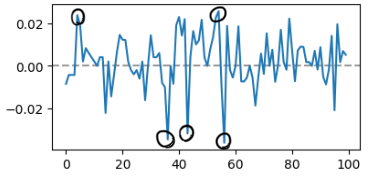
\includegraphics[scale = 0.7]{imgs/small_peaks.png}
        \captionof{figure}{}
        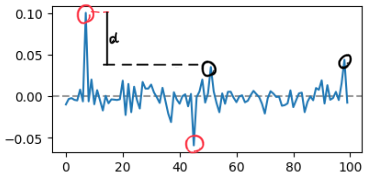
\includegraphics[scale = 0.7]{imgs/big_peaks.png}\\
        \captionof{figure}{}
    \end{center}
    As we can see the in (\textbf{Figure 1}) the 2 highest peaks are not very far from each other. This makes the order of magnitude lower compared to the peak we can see in the (\textbf{Figure 2}). Let's analyze two different meanings a peak can refer to:
    \begin{itemize}
        \item a strong movement in price
        \item a shock, due to news or particural events.
    \end{itemize}  
    Taking into consideration the nature of the sample taken, it is very unlikely to have two big shocks in the same window. Following this logic, when the $1^{st}$ and $2^{nd}$ peaks in a series are close, we can conclude they are probably just strong movements in the price. Again, when the $1^{st}$ peak in terms of magnitude is way bigger than the $2^{nd}$, it is unlinkely to have price movements with this elevated magnitude, in very small ranges. We can note that since the usual price movement of these kind of stocks falls between a range of -0.01\% and 0.01\%, It seems reasonable to apply the scaler function to get an ultimate generated series that can be used for data analysis purposes while reflecting the true nature of the financial asset. 
    \subsection*{Scaler Logic}
    Following this reasoning, the scaler assigns the value that shocks typically have in real data, to isolated peaks in the generated series, adjusting it to a value plausible in real scenarios.
    It also assigns values typical for strong market movements to peaks very close to each other.
    \subsection*{Scaler Implementation}
    The scaler computes the quantiles of the maximum values in the distribution and for the distribution of the difference between the $1^{st}$ and 
    $2^{nd}$ peaks.\\
    Then the algorithm computes the distance between the $1^{st}$ and $2^{nd}$ peaks in the sample compared to the quantiles of the differences for real 
    data. A random value is then sampled from a uniform distribution where the lower and upper bonuds are the corresponding quantiles in the maximum distribution. 
    The same functions are applied to the negative peaks.
    \end{multicols}
    \textbf{Exemple:}
    \begin{center}
        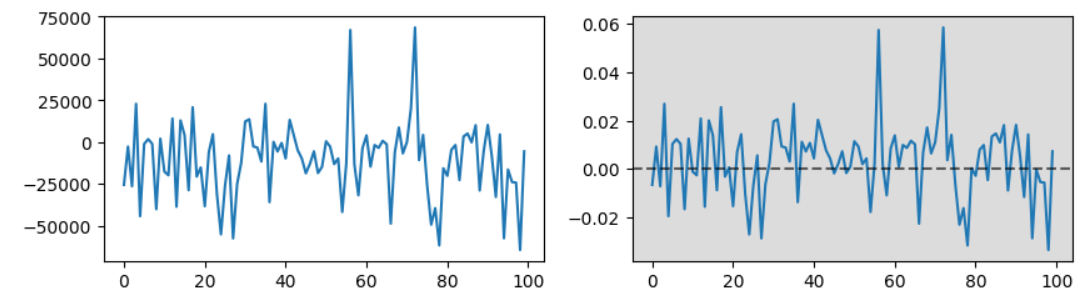
\includegraphics[scale=0.6]{imgs/EX_03.png}
    \end{center}
    In the above exemple on the left we can see the series our model generated and on the right the series after the scaler is applied. As we can see,  
    the scaler preserves the pattern generated by our model but rescales the data such that we have realistic data we can use for other experiments and implementations.



\begin{center}
    {\huge{Filter}}
\end{center}    
    \begin{multicols}{2}
    \section*{Problem}
    One problem we noticed in the samples our model generated after the application of the scaler is, that some are decent and realistic, but others are 
    nonsense, as is illustrated in the exemples below:
    \begin{center}
        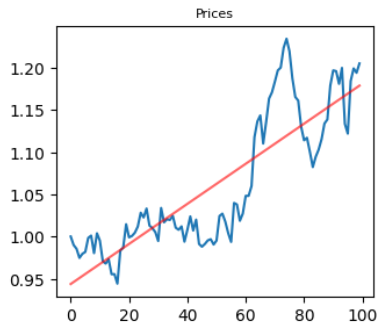
\includegraphics[scale=0.49]{imgs/serie_comp_1.png}
        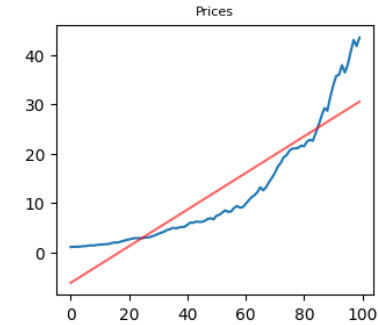
\includegraphics[scale=0.49]{imgs/serie_comp_2.png}
    \end{center}
    As we can see, the first series is realistic but the other one is not only out of scale but shows a trendline that is very 
    atypical for fiancial time series. In order to solve this problem, we created a filter that selects from the samples generated the realistic series without modifyng the model output, that way we end up with a realistic series dataset.
    \section*{How It works}
    To select the realistic series we came up with several metrics, the value of which can be tuned in the filter parameters:
    \paragraph*{Distance between residuals.}
    We noticed that if we apply a linear regression to a series, the distance between consecutive residuals is significantly smaller when the series shows an unrelistic behavior.
    In contrast, for more realistic series the discance between consecutive points residuals is bigger.
    \begin{center}
        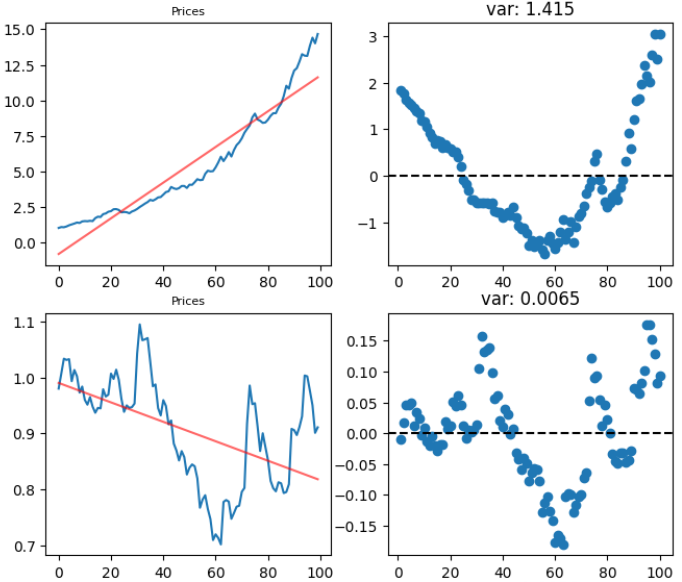
\includegraphics[scale=0.6]{imgs/2_res.png}
    \end{center}
    We scaled the price of the generated series to the range form 0 to 1 to in order to make it comparable. Then we applied linear regression and computed the sum of the distance between consecutive residuals. 
    Then the filter just selects the series with a sum of consecutive residuals above a given threshold.\\
    \textbf{DfGenerator parameter}:  \textbf{variance\_th}.
    \paragraph*{Maximum range of oscillation}
    We decided to introduce a parameter in the filter to chose the maximum range of oscillation between the first point an the last one in percentage. This is because we think it could be useful to have the freedom to decide the type of series we want 
    to generate to expand our dataset. Potentially we would want to expand our dataset with very volatile series, in which case we can chose to use a high maximum range of osscilation. Alternatively, our need could be to expand our dataset with more stable series, for example in order to decrease 
    the volatility of the predictions made by a model. In that case we can tune the parameter chosing a lower maximum range.\\
    \textbf{DfGenerator parameter}:  \textbf{max\_range}.

    \end{multicols}
    \newpage
    \begin{center}
        {\huge{Final Results}}
    \end{center} 
    The final result of the project is a program capable of generating seemingly realistic financial series such the following:
    \begin{center}
        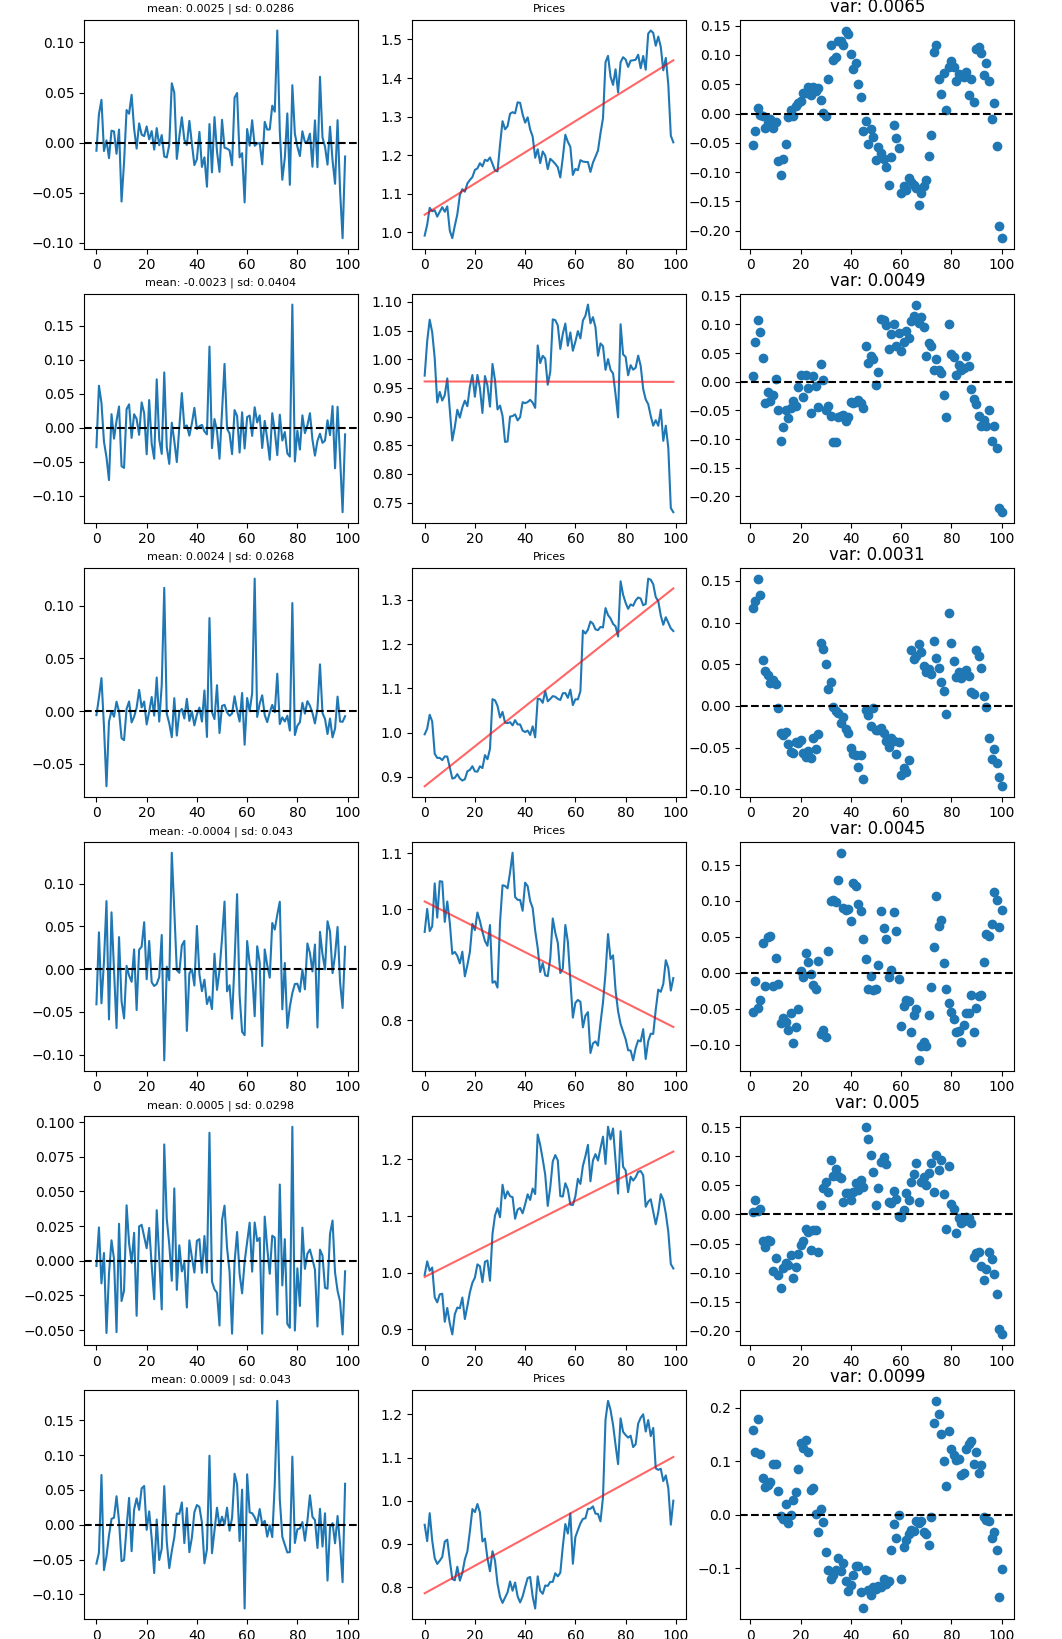
\includegraphics[scale=0.5]{imgs/results_reduced.png}
    \end{center}
    \newpage
    The generated series are visually similar to the original series. In the graph, the generated series have a grey background to distinguish them from the original ones:
    \begin{center}
        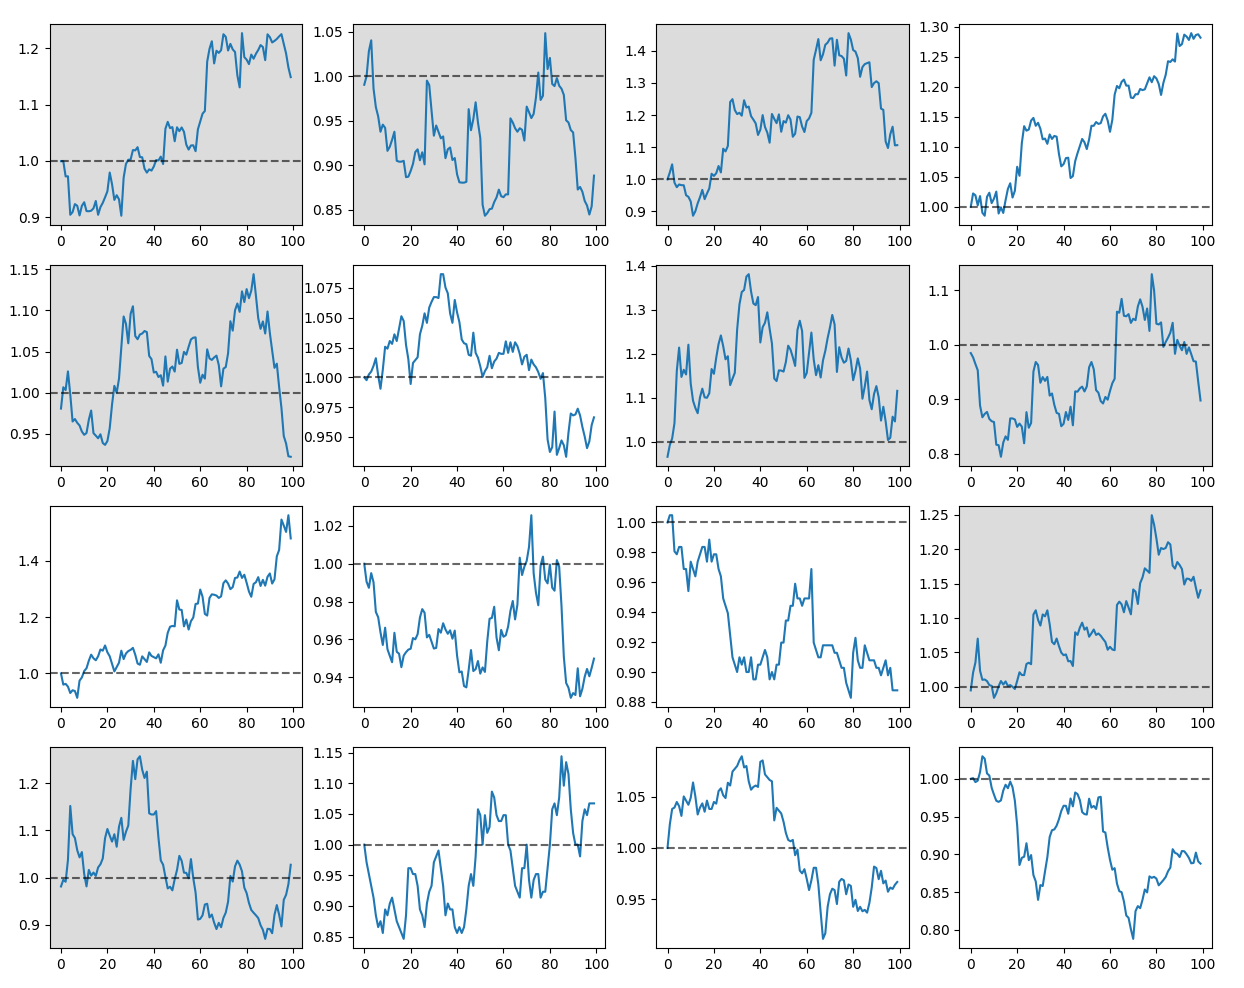
\includegraphics[scale=0.3]{imgs/series_comparison_README.png}
    \end{center}
    One of the main characteristics of returns of financial products is that the mean is almost equal to 0. We tested if the mean of the returns generated by our model and the mean 
    of the real series of the dataset is the same. If the generated series are relaistic, they should follow the same distribution, lead to the following hypotesis test:
    \begin{equation}
        \begin{cases}
        H_0: \;\; \overline{X}=0\\
        H_1: \;\; \overline{X} \neq 0
    \end{cases}\,.
    \end{equation}
    $$T=\frac{\overline{X}-\mu_0}{S_n/\sqrt{n}} \;\;\;\;\;\;\;\;\;\;\; T|H_0 \sim t_{n-1}$$
    We test this hypothesis on a generated a dataset of 10 000 samples, which yields computed mean of 0.00026567.
    The program takes approximatly 20 mintutes to generate a 10 000 samples dataset on a single CPU Intel Core I7. The means of the generated samples are distributed as follows:
    \begin{center}
        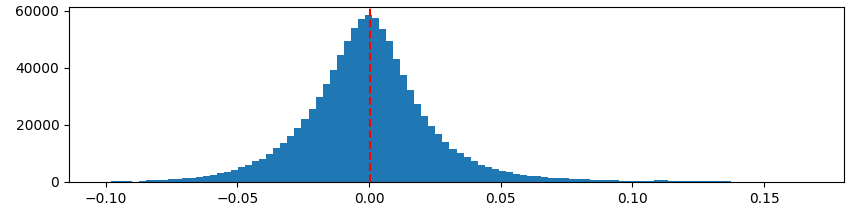
\includegraphics[scale=0.7]{imgs/generated.png}
    \end{center}
    
    \newpage
    \begin{center}
        {\huge{Future Work}}
    \end{center} 
    This is a list of future work improving upon our project:
    \begin{enumerate}
        \item Develop a robust testing framework to evaluate generated time series datasets
        \item Test and compare a wider set of architectures
        \item Implement a tensorboard interface to check model performance in realtime during the training
        \item Inlcude the rescaler in the model architecture of the generator such that the quantiles can be optimized during the training or get completely rid of the need for it
        \item Test the models performance on different types of datasets (e.g. specific sectors stocks) to see how this affects the results
        \item study the statistical properties of the series generated
        \item Expand a datataset and see how this affects the performance of a prediction model
    \end{enumerate}

    % \cite{Mindermann_2022}
    
    \begin{thebibliography}{9}
        \bibitem{Mindermann_2022}
        Mindermann, S., et al. (2022) \emph{Prioritized Training on Points that are learnable, Worth Learning, and Not Yet Learnt.}, \href{https://doi.org/10.48550/arXiv.2206.07137}{arXiv.2206.07.137}.
        
        \bibitem{}
        \end{thebibliography}

\end{document}
